\documentclass{article}

% Use preprint so the author block is visible for the class report.
\usepackage[preprint]{neurips_2025}

\usepackage[utf8]{inputenc}
\usepackage[T1]{fontenc}
\usepackage{hyperref}
\usepackage{url}
\usepackage{booktabs}
\usepackage{amsfonts}
\usepackage{amsmath}
\usepackage{nicefrac}
\usepackage{microtype}
\usepackage{xcolor}
\usepackage{graphicx}
\usepackage{array}

\title{Do Medical QA Benchmarks Measure Medically Grounded Reasoning? \\
A Natural Language Autoencoder Study of Latent Explanations}

\author{%
  Blake Masters \\
  Department of Computer Science / Department of Bioengineering and Therapeutic Sciences\\
  Stanford University / University of California - San Francisco\\
  \texttt{blakemasters@stanford.edu} \\
}

\newcommand{\runpath}{\texttt{runs/vast\_final\_report/38347984\_final/report\_qwen\_medqa\_n200}}
\newcommand{\scorerheuristic}{\texttt{heuristic\_v1}}
\newcommand{\scorerjudge}{\texttt{medgemma\_judge\_v1}}

\begin{document}

\maketitle

\begin{abstract}
Medical multiple-choice question answering benchmarks are often reported as evidence that a language model has acquired medically grounded reasoning. Final-answer accuracy is useful, but it is an incomplete measurement of that construct: a model may answer correctly through memorization, option artifacts, or shallow associations. This report evaluates whether Natural Language Autoencoder (NLA) explanations can provide auxiliary validity evidence for medical QA evaluation. I ran a final-scale experiment on 200 MedQA questions with Qwen2.5-7B-Instruct, three prompt variants per question, layer-20 activation probes, NLA verbalization and reconstruction, heuristic rationale scoring, and a MedGemma 4B automated judge. The run produced 600 predictions, 600 decoded NLA explanations, and 1,200 score records across the two scorers. Validation passed with a 100\% decode parse rate, zero CJK injection warnings, and mean reconstruction cosine 0.828. The model's answer accuracy was 57.5\%. However, the estimated rate of aligned latent explanations depended strongly on the scorer: 5.5\% under a strict lexical heuristic and 77.7\% under the MedGemma judge. This discrepancy is the central finding. NLA explanations appear useful as a measurement instrument for auditing medical QA behavior, but automated explanation scoring is itself a major source of measurement uncertainty. The results should therefore be read as single-model, single-dataset validity evidence rather than as proof that NLA explanations reveal literal model reasoning.
\end{abstract}

\section{Introduction}

Medical QA benchmarks provide a compact way to evaluate open-weight language models on clinical and biomedical knowledge. A common reporting pattern is to treat multiple-choice accuracy as a proxy for medical reasoning ability. That proxy is imperfect. A correct answer can arise from medically grounded reasoning, memorized exam patterns, answer-option artifacts, or other shortcuts. Conversely, an incorrect answer can coexist with partially relevant medical representations. This creates a construct validity problem: the observed benchmark score does not fully measure the latent capability of interest.

This project is directly motivated by the original Natural Language Autoencoders work, which introduced the idea of translating internal model activations into natural language and reconstructing the activation from that text \citep{anthropic2026nla, kitft2026nla}. Because this report applies that method almost directly to a medical QA measurement question, the NLA work is the closest methodological antecedent rather than a distant background citation.

The project asks whether NLA explanations can serve as auxiliary measurements for medically grounded reasoning. NLAs decode internal activations into natural-language text and can optionally reconstruct the activation from that text. In this report, the NLA explanation is not treated as direct access to model thoughts. It is treated as an imperfect measurement instrument that may reveal whether the activation at a specific point contains medically relevant information aligned with the benchmark problem.

The original proposal considered two NLA-supported base models and two medical QA datasets. The completed final run was narrowed for compute and time: it evaluates Qwen2.5-7B-Instruct on 200 MedQA items, using three prompt variants for each item. This narrower scope is still sufficient to test the project pipeline end to end and to answer a focused measurement question:

\begin{quote}
\textbf{When Qwen2.5-7B-Instruct answers MedQA questions, how often do NLA-decoded latent explanations appear medically aligned, and how does that compare with final-answer accuracy?}
\end{quote}

The main contribution is a reproducible measurement pipeline and a first empirical estimate of the gap between answer accuracy and latent-explanation alignment under two automated scoring rules. The result is not a clinical safety claim or a general benchmark claim. It is an audit of one model, one dataset, and one NLA checkpoint family.

\section{Related work}

MedQA is a multiple-choice OpenQA dataset derived from professional medical board exams \citep{jin2020medqa}. It is useful for construct-validity analysis because questions are designed to measure applied medical knowledge, while model outputs are still reduced to discrete answer options. MedMCQA offers a larger multi-subject medical QA benchmark with richer subject coverage \citep{pal2022medmcqa}, but it was not included in the completed final run.

Recent medical QA evaluation work has argued that explanations matter in addition to final answers. MedExQA, for example, criticizes pure classification accuracy as insufficient for assessing nuanced medical understanding and evaluates medical explanations as part of QA assessment \citep{kim2024medexqa}. This report follows the same broad motivation, but uses decoded activations rather than model-generated post hoc rationales.

Natural Language Autoencoders provide a method for mapping model activations to natural-language descriptions and then reconstructing activations from those descriptions. The released NLA inference code and checkpoints support several open-weight instruction models, including Qwen2.5-7B-Instruct at layer 20 \citep{anthropic2026nla, kitft2026nla}. This makes it possible to ask whether a hidden activation associated with a medical QA prompt contains information that an independent decoder renders as medically meaningful text.

\section{Methods}

\subsection{Data, model, and prompt variants}

The experiment used 200 English MedQA test items sampled from the Hugging Face dataset \texttt{GBaker/MedQA-USMLE-4-options}. Each item has a question, four answer choices, and a correct answer key. The base model was Qwen2.5-7B-Instruct, evaluated in greedy answer mode. For each item, the pipeline rendered three prompt variants: a canonical format, a compact format, and an option-shuffle format. This produced 600 prompt-variant prediction records.

For each prompt, the model generated a short answer, the answer parser normalized the selected option, and correctness was computed against the original answer key after reversing any variant-specific option mapping. This matters for prompt stability: a shuffled variant can change the displayed option letter while preserving the original answer identity.

\subsection{Activation probing and NLA decoding}

For each prompt-variant record, the pipeline extracted the residual activation from the configured decoder layer at the pre-answer last prompt token. Operationally, the token index was computed from the attention mask length, and the raw activation vector was stored without normalization. The Qwen NLA sidecar specifies a hidden width of 3,584 at layer 20.

The activation verbalizer was \texttt{kitft/nla-qwen2.5-7b-L20-av}, served with SGLang. The activation reconstructor was \texttt{kitft/nla-qwen2.5-7b-L20-ar}. The decoder extracted explanations from \texttt{<explanation>...</explanation>} tags and computed reconstruction cosine and mean squared error when the reconstructor was enabled. The final run used the critic, so reconstruction metrics are available.

\subsection{Scoring and taxonomy}

Each decoded explanation was scored by two automated scorers. The heuristic scorer uses deterministic lexical and support rules. It is intentionally conservative: it rewards explicit overlap with medical terms and selected-answer support, and it can label many semantically plausible explanations as weak if the lexical evidence is not present.

The MedGemma judge scorer uses \texttt{google/medgemma-4b-it} with a locked JSON rubric. It emits fields for medical relevance, rationale alignment, answer support, shortcut suspicion, medically invalid reasoning, and a binary NLA quality label. The parser is strict: malformed JSON or schema violations are converted into failure score records rather than silently coerced. The final judge run scored 600 rows and reported 46 strict-parse failures. These failures are included in the scored file and are discussed as judge reliability limitations.

For both scorers, each prediction is assigned to one of four cells:

\begin{center}
\begin{tabular}{lll}
\toprule
Answer correctness & Explanation quality & Interpretation \\
\midrule
Correct & Aligned & Stronger evidence of medically grounded answer selection \\
Correct & Weak & Possible shortcut, memorization, or incomplete latent explanation \\
Incorrect & Aligned & Medical content present despite final answer failure \\
Incorrect & Weak & Broader failure of answer and decoded explanation \\
\bottomrule
\end{tabular}
\end{center}

\subsection{Validation and uncertainty}

All reported metrics were computed from the final artifact directory \runpath. The run validator checked item, prediction, decode, and score joins; required output files; decode parse rate; CJK warning counts; taxonomy validity; and score coverage. Bootstrap intervals in the analysis tables resample item IDs as blocks, preserving the three prompt-variant records for each item.

\section{Results}

\subsection{Run validation}

The final run produced the intended artifact set: 200 items, 600 predictions, 600 NLA decodes, 600 heuristic score records, 600 MedGemma judge score records, analysis tables, validation output, and a report bundle. The validator returned \texttt{ok: true}. All decoded records parsed successfully, no CJK injection warnings were emitted, and the mean reconstruction cosine was 0.828. Table~\ref{tab:run-summary} summarizes the run.

\begin{table}[t]
\caption{Final run summary. Counts are from the validated final artifact directory.}
\label{tab:run-summary}
\centering
\begin{tabular}{ll}
\toprule
Quantity & Value \\
\midrule
Dataset & MedQA test subset \\
Model & Qwen2.5-7B-Instruct \\
NLA layer & 20 \\
Items & 200 \\
Prompt variants per item & 3 \\
Prediction and decode records & 600 \\
Scored records & 1,200 across two scorers \\
Decode parse-ok rate & 100\% \\
CJK injection warnings & 0 \\
Mean reconstruction cosine & 0.828 \\
Mean reconstruction MSE & 0.343 \\
\bottomrule
\end{tabular}
\end{table}

\subsection{Accuracy and aligned-explanation rates}

Answer accuracy was 57.5\% across the 600 prompt-variant records, with item-bootstrap 95\% interval 51.5\% to 63.8\%. The aligned-explanation rate varied sharply by scorer. The heuristic scorer labeled only 5.5\% of records as aligned, while the MedGemma judge labeled 77.7\% as aligned. This is shown in Table~\ref{tab:summary} and Figure~\ref{fig:accuracy-alignment}.

\begin{table}[t]
\caption{Accuracy and aligned-explanation rates by scorer. Confidence intervals are item-bootstrap intervals from the analysis stage.}
\label{tab:summary}
\centering
\begin{tabular}{lrrrr}
\toprule
Scorer & Accuracy & 95\% CI & Aligned rate & 95\% CI \\
\midrule
Heuristic & 57.5\% & [51.5, 63.8]\% & 5.5\% & [3.2, 8.2]\% \\
MedGemma judge & 57.5\% & [51.5, 63.8]\% & 77.7\% & [73.5, 81.3]\% \\
\bottomrule
\end{tabular}
\end{table}

\begin{figure}[t]
\centering
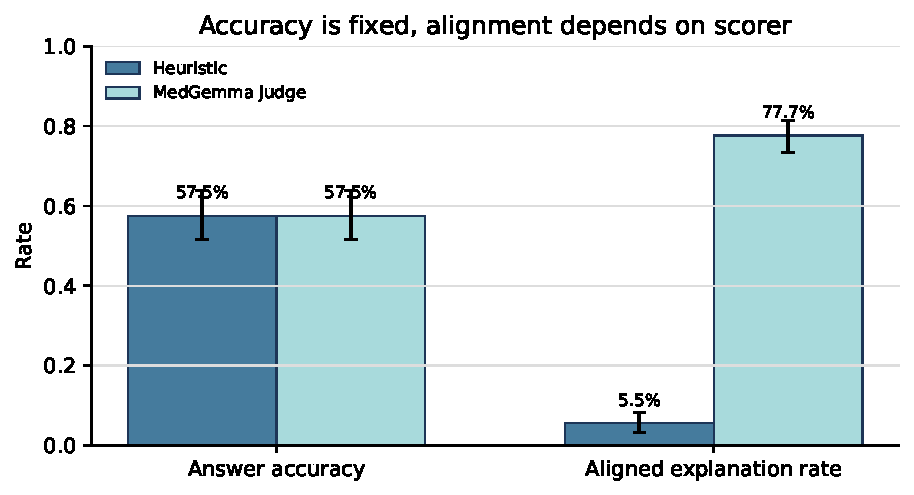
\includegraphics[width=0.72\linewidth]{figures/accuracy_alignment.pdf}
\caption{Final-answer accuracy is independent of the explanation scorer, while the estimated aligned-explanation rate is highly scorer-dependent. Error bars are item-bootstrap intervals.}
\label{fig:accuracy-alignment}
\end{figure}

This scorer disagreement is not a minor implementation detail. It changes the substantive interpretation. Under the heuristic scorer, most correct answers are classified as correct but weak. Under the MedGemma judge, most correct answers are classified as correct and aligned. The difference suggests that automated explanation evaluation is itself a high-variance measurement step. A strict lexical scorer may have low recall for semantically relevant explanations, while an LLM judge may be more permissive or influenced by the answer and question context.

\subsection{Correctness crossed with latent-explanation quality}

Table~\ref{tab:taxonomy} and Figure~\ref{fig:taxonomy} show the four-cell taxonomy. Under the MedGemma judge, 317 of 600 records were correct and aligned, while 28 were correct but weak. There were also 149 incorrect but aligned records, suggesting cases where the decoded activation contained medically relevant content even though answer selection failed. Under the heuristic scorer, the dominant cells were correct weak and incorrect weak, consistent with a conservative overlap rule.

\begin{table}[t]
\caption{Taxonomy counts and rates by scorer. Rates are over 600 prompt-variant records.}
\label{tab:taxonomy}
\centering
\small
\begin{tabular}{lrrrr}
\toprule
Scorer & Correct aligned & Correct weak & Incorrect aligned & Incorrect weak \\
\midrule
Heuristic & 27 (4.5\%) & 318 (53.0\%) & 6 (1.0\%) & 249 (41.5\%) \\
MedGemma judge & 317 (52.8\%) & 28 (4.7\%) & 149 (24.8\%) & 106 (17.7\%) \\
\bottomrule
\end{tabular}
\end{table}

\begin{figure}[t]
\centering
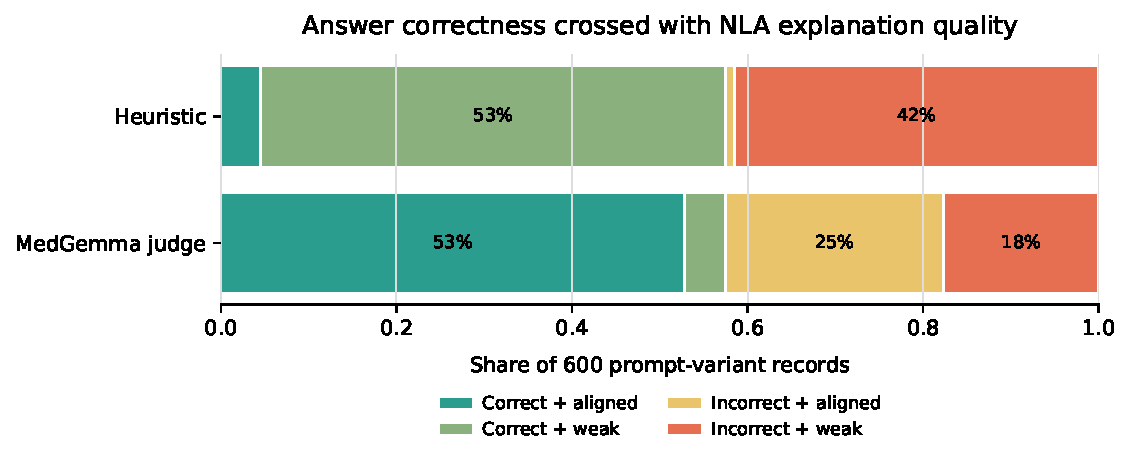
\includegraphics[width=0.78\linewidth]{figures/taxonomy_stack.pdf}
\caption{The four-cell taxonomy changes substantially with the scoring instrument. The heuristic emphasizes weak explanations; the MedGemma judge identifies many aligned explanations among both correct and incorrect answers.}
\label{fig:taxonomy}
\end{figure}

The MedGemma taxonomy supports a more nuanced reading than accuracy alone. Accuracy says that the model selected the correct answer in 57.5\% of prompt-variant records. The taxonomy splits that result into cases where the decoded activation appears aligned and cases where it does not. It also identifies incorrect-but-aligned cases, which are important because they separate medical content in the activation from the final answer selection mechanism. However, because the judge itself has parse failures and no human-adjudicated labels in this run, these should be treated as candidate audit categories rather than final clinical judgments.

\subsection{Reconstruction and prompt stability}

Reconstruction quality was stable across taxonomy cells. Mean reconstruction cosine values ranged from roughly 0.826 to 0.843 across the scorer-cell combinations, with an overall mean of 0.828. Figure~\ref{fig:reconstruction} shows that cell membership was not driven by large reconstruction-quality differences. This is useful because it reduces one simple confound: the weak categories do not merely reflect failed NLA reconstruction.

\begin{figure}[t]
\centering
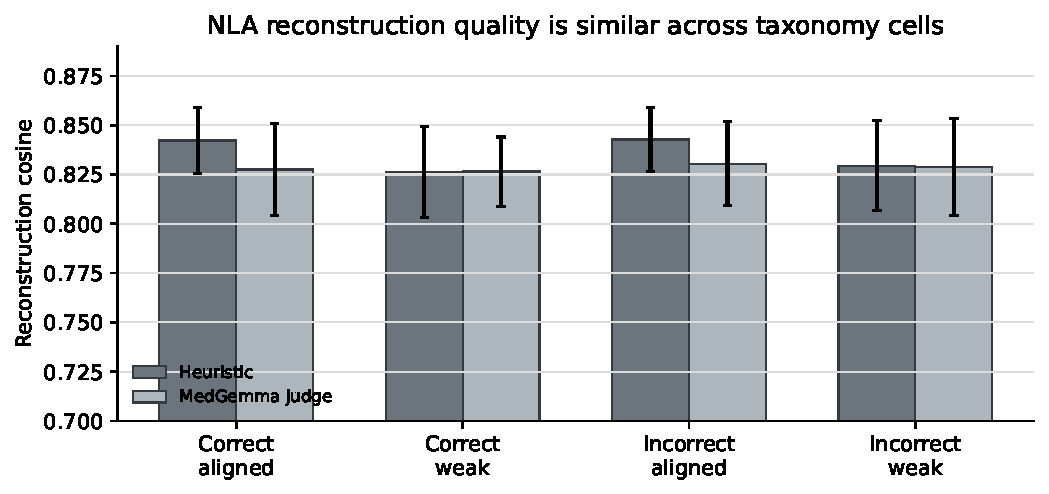
\includegraphics[width=0.80\linewidth]{figures/reconstruction_by_cell.pdf}
\caption{Mean reconstruction cosine by taxonomy cell. Error bars show the observed standard deviation within each cell. Reconstruction quality is similar across cells, so the taxonomy differences mainly reflect scoring behavior rather than gross reconstruction failure.}
\label{fig:reconstruction}
\end{figure}

Prompt stability was moderate. Across 200 items, the mean answer agreement across the three prompt variants was 0.775, and 37 items had a changed original-answer identity under the option-shuffle variant. Correctness agreement averaged 0.835. Explanation-quality agreement was scorer-dependent: 0.905 for the heuristic scorer and 0.600 for the MedGemma judge. This again points to scoring sensitivity. The answer parser and variant remapping make it possible to detect prompt instability, but a larger run would be needed to estimate subject-level effects.

\section{Qualitative audit signals}

The report bundle generated an 80-row manual audit queue. The queue intentionally prioritizes correct-weak failure cases, prompt-instability cases, and taxonomy coverage. Because no human labels have been added yet, these rows are not presented as adjudicated errors. They are examples of where a human reviewer should inspect the decoded explanation, gold answer, selected answer, and scorer evidence.

The highest-priority automated failure cases often had a recognizable pattern: the model selected the correct answer, while the decoded explanation described prompt format, answer position, or an incoherent answer cue rather than a medically grounded mechanism. For example, some decoded explanations referred to generic ``Q\&A'' structure or to the answer token itself. These cases are exactly why the NLA audit is useful: they are correct under benchmark accuracy, but the auxiliary explanation signal suggests weaker validity evidence for medically grounded reasoning.

\section{Discussion}

The completed run supports three conclusions. First, the pipeline is technically viable. It produced base-model predictions, raw activations, NLA decodes, reconstruction metrics, two score files, analysis outputs, validation output, and a report bundle for a 200-item MedQA subset.

Second, answer accuracy alone hides meaningful heterogeneity. A 57.5\% accuracy score does not distinguish between correct answers with aligned latent explanations and correct answers where the decoded activation appears weak or shortcut-like. Under the MedGemma judge, most correct answers were aligned, but a small set remained correct weak. Under the heuristic scorer, most correct answers were weak, showing that the measurement conclusion depends heavily on the scoring instrument.

Third, scorer design is the dominant unresolved validity issue. The heuristic scorer is transparent and reproducible, but probably under-recognizes semantic medical relevance. The MedGemma judge is more semantically flexible and produces evidence text, but it is an automated LLM judge with 46 strict-parser failures in this run. Without human adjudication, the two scorers should be interpreted as bracketing plausible measurement behavior rather than as definitive labels.

\section{Limitations}

The most important limitation is scope. The original plan included Gemma-3-12B-IT and MedMCQA; the final report includes only Qwen2.5-7B-Instruct on MedQA. This prevents cross-model or cross-dataset claims. The sample size is also a subset rather than the full benchmark, though the run includes prompt variants and item-bootstrap intervals.

The second limitation is the interpretation of NLA explanations. NLAs are trained measurement instruments, not ground-truth windows into cognition. A decoded explanation can be incomplete, distorted, or biased toward the verbalizer's training distribution. Reconstruction cosine helps detect gross failures, but high reconstruction quality does not prove semantic faithfulness.

The third limitation is automated scoring. The heuristic and MedGemma judge disagree sharply. This is useful evidence about measurement uncertainty, but it means the aligned-rate estimates should not be treated as final. A small human audit is the natural next step, especially for correct-weak, incorrect-aligned, and prompt-instability cases.

\section{Conclusion}

This project reframes medical QA evaluation as a measurement problem. In the completed Qwen2.5-7B-Instruct MedQA run, answer accuracy was 57.5\%, but auxiliary NLA-based explanation measurements showed that the interpretation of correctness depends on how latent explanations are scored. The MedGemma judge found many aligned explanations, including among incorrect answers, while the stricter heuristic found few. The central lesson is therefore not that NLA explanations replace benchmark accuracy. Instead, they provide an additional audit channel that can expose cases where final-answer scores are under-informative and where explanation-scoring choices materially affect validity claims.

\section*{Reproducibility statement}

All reported results are sourced from \runpath. The run used Qwen2.5-7B-Instruct, the Qwen layer-20 NLA actor and critic, SGLang decode, heuristic scoring, MedGemma 4B judge scoring, item-bootstrap analysis, run validation, and report-bundle export. The validator passed with \texttt{ok: true}. The report intentionally avoids claims about models, datasets, or clinical settings that were not included in the completed run.

\section*{Required disclosures}

\paragraph{Plagiarism, bias, and accuracy.}
I addressed plagiarism risk by writing the report in my own words, citing the original NLA work and the medical QA datasets where their ideas, methods, or data shaped the project. I avoided presenting NLA explanations as my invention and distinguished my contribution from the released NLA checkpoints and inference code. To reduce bias and inaccuracy, I reported the completed scope rather than the broader original proposal, preserved negative and ambiguous findings, and stated that the automated scorers disagree substantially. I checked all numerical claims against the generated artifacts and validation files. I also avoided clinical recommendations and treated MedQA items as benchmark data rather than patient-specific evidence. Remaining risks include automated judge bias, dataset bias, and possible errors in NLA interpretation; these are described as limitations rather than hidden or converted into stronger claims. I checked phrasing against source boundaries so dataset descriptions, methods, and claims remained visibly attributed throughout.

\paragraph{AI tool use reflection.}
I used generative AI tools as coding, debugging, execution-planning, and drafting assistants throughout the project. They helped implement the data pipeline, inspect logs, prepare Vast runs, summarize artifacts, generate draft report language, and identify consistency checks. I treated their outputs as provisional work products rather than authoritative answers. For code, I ran tests and validation scripts; for the report, I checked claims against the saved experiment artifacts. The main learning impact was practical: AI tools made it possible to move faster through infrastructure details while forcing me to define interfaces, tests, assumptions, and failure criteria more explicitly. In future work, I would use AI tools similarly for scaffolding and audit support, but I would continue to keep final responsibility for scientific framing, attribution, statistical interpretation, and claims. This division kept the tools useful for acceleration while leaving interpretation, prioritization, and responsibility with me as the responsible researcher and final author.

\paragraph{Impact statement.}
This work could improve medical AI evaluation by showing where benchmark accuracy may be incomplete evidence of medically grounded reasoning. It could also be misused if NLA explanations or automated judge labels are treated as proof of clinical reliability. To mitigate that risk, the report states that NLA outputs are auxiliary measurements, not literal model thoughts or clinical explanations, and it avoids making deployment claims. The environmental impact comes mainly from GPU inference; I limited the final run to a modest 200-item sample after pilot tests and recorded artifact-level evidence rather than rerunning unnecessarily. The data are public benchmark questions, not human-subject or patient-identifiable records. I followed academic integrity standards by citing related work, reporting scope reductions, preserving limitations, and distinguishing automated scoring from human medical review. If these methods inform future medical evaluation, they should be paired with human review and transparent uncertainty reporting before use in higher-stakes settings elsewhere.

{\small
\begin{thebibliography}{9}

\bibitem[Anthropic(2026)]{anthropic2026nla}
Anthropic. 2026.
\newblock Natural Language Autoencoders: Turning Claude's thoughts into text.
\newblock \url{https://www.anthropic.com/research/natural-language-autoencoders}.

\bibitem[Jin et~al.(2020)]{jin2020medqa}
Jin, Di, Pan, Eileen, Oufattole, Nassim, Weng, Wei-Hung, Fang, Hanyi, and Szolovits, Peter. 2020.
\newblock What Disease does this Patient Have? A Large-scale Open Domain Question Answering Dataset from Medical Exams.
\newblock \emph{arXiv preprint arXiv:2009.13081}.

\bibitem[Kim et~al.(2024)]{kim2024medexqa}
Kim, Yubin, Pal, Surjodeep, Choi, Jong Hyun, and Lee, Hyunjae. 2024.
\newblock MedExQA: Medical Question Answering Benchmark with Multiple Explanations.
\newblock \emph{arXiv preprint arXiv:2406.06331}.

\bibitem[kitft(2026)]{kitft2026nla}
kitft. 2026.
\newblock Natural Language Autoencoders and NLA inference repositories.
\newblock \url{https://github.com/kitft/natural_language_autoencoders} and \url{https://github.com/kitft/nla-inference}.

\bibitem[Pal et~al.(2022)]{pal2022medmcqa}
Pal, Ankit, Umapathi, Logesh Kumar, and Sankarasubbu, Malaikannan. 2022.
\newblock MedMCQA: A Large-scale Multi-Subject Multi-Choice Dataset for Medical domain Question Answering.
\newblock \emph{Proceedings of the Conference on Health, Inference, and Learning}, PMLR 174:248--260.

\end{thebibliography}
}

\end{document}
